% Document class and packages
\documentclass[a4paper, 12pt]{report}
\usepackage{geometry}
\usepackage[utf8]{inputenc}
\usepackage{graphicx}
\usepackage{titlesec}
\usepackage{fontenc}
\usepackage{float}
\usepackage{minted}
\usepackage[swedish]{babel}
\usepackage{pythonhighlight}
\usepackage{wrapfig}
% For headers and footers
\usepackage{fancyhdr, lastpage}
\usepackage{fancyvrb}
% Math spesific packages
\usepackage{amsfonts}
\usepackage{amsmath}
\usepackage{amssymb}
% For reffereces displaying and coloring as well as for some document settings
\usepackage[]{hyperref}
% For math symbols and figures
\usepackage{tikz}
% For color boxes
\usepackage{xcolor}
\usepackage[most]{tcolorbox}
% For unit displaying
\usepackage{siunitx}
% For correct paragraph phrasing
\usepackage{parskip}

% For figure caption formatting
\usepackage[font=small,labelfont=bf,center]{caption}

% For correct fotnotes and citation structure
\usepackage[backend=bibtex8,style=verbose,citestyle=alphabetic,bibstyle=alphabetic]{biblatex}
\addbibresource{ref.bib}

% Background image of title page
\usepackage{eso-pic}
\newcommand\BackgroundIm{
\put(0,0){
\parbox[b][\paperheight]{\paperwidth}{
\vfill
\centering

\includegraphics[height=\paperheight,width=\paperwidth,
keepaspectratio]{background-1.png}
\vfill
}}}

% To fix footnote counter between files
\usepackage{chngcntr}
\counterwithout*{footnote}{chapter}

% Global options
\geometry{a4paper}
\graphicspath{{Images/}}
\hypersetup{
  linkcolor=black,
  citecolor={blue!50!black},
  filecolor={blue!50!black},
  urlcolor={blue!80!black},
  pdftitle={The AES encryption algorithm},
  pdfauthor={Gabriel Lindeblad},
  pdfcreator={Gabriel Lindeblad},
  pdfsubject={Advanced Encryption Standard},
  pdfstartpage=1,
  pdffitwindow=true,
  colorlinks=true,
  pdfpagemode=UseNone,
  }
\setcounter{tocdepth}{3}
\setcounter{secnumdepth}{3}
\pagestyle{fancy}
\rhead{\currentchapter}
\cfoot{\thepage}
\fancyheadoffset[L, RO]{0cm}


% New commands and changed commands
\newcommand{\currentchapter}{}
\newcommand{\mychapter}[1]{\chapter{#1}
\renewcommand{\currentchapter}{#1}}
\renewcommand{\bibname}{Källförteckning}
\renewcommand{\contentsname}{Inehållsförteckning}
\addto\captionsswedish{%
  \renewcommand\listfigurename{Figur lista}}
\newcommand{\fakechapter}[2]{%
  \par\setcounter{chapter}{#2}
  \chaptermark{#1}
  \rhead{ }
}
\newcommand*{\captionsource}[2]{%
  \caption[{#1}]{%
    #1%
    \\\hspace{\linewidth}%
    \textbf{Källa:} #2%
  }%
}

% Titel reformating
\titleformat{\chapter}[block]
  {\normalfont\huge\bfseries}{\thechapter}{0.5em}{\Huge}
\titlespacing*{\chapter}{0pt}{-25pt}{0pt}

\titleformat{\section}[block]
  {\normalfont\Large\bfseries}{\thesection}{0.5em}{\Large}
\titlespacing*{\chapter}{0pt}{-25pt}{0pt}

\titleformat{\subsection}[block]
  {\normalfont\large\bfseries}{\thesubsection}{0.5em}{\large}
\titlespacing*{\chapter}{0pt}{-25pt}{0pt}

\titleformat{\subsubsection}[block]
  {\normalfont\normalsize\bfseries}{\thesubsubsection}{0.5em}{\normalsize}
\titlespacing*{\chapter}{0pt}{-25pt}{0pt}


% Glossaries setup
\usepackage[nopostdot,nonumberlist,style=altlisthypergroup,acronym,toc]{glossaries}
\makeglossaries

\renewcommand*{\glossaryname}{Begreppförklaring}
\renewcommand*{\acronymname}{Akronymer}
\renewcommand{\glsnamefont}[1]{\textbf{#1}}

%%%
\newglossaryentry{rsa}
{
    name={RSA},
    description={Rivest-Shamir-Adleman (RSA) är en av det mest välkända krypteringsalgoritmerna
    och var en av det första algoritmerna som byggde på en asymmetrisk kryptering.
    RSA bygger på multiplikation av stora primtal där primtalen är
    nycklarna.\cite{rsa-ref}}
 }

\newglossaryentry{caesar}
{
    name={Caesarchiffer},
    description={Caesarchiffer är ett \gls{substitutionsskiffer},
    vilket helt enkelt bygger på att man byter ut varje bokstav i
    meddelandet med en annan. Ersättnings bokstaven bestäms genom
    att man hoppar ett visst antal hopp i alfabetet som exempelvis
    3 hopp, vilket då innebär att ifall man har bokstaven a då skulle
    den bli ett d istället.\cite{caesar}}
 }

\newglossaryentry{xor}
{
    name={XOR},
    symbol={\(\oplus\)},
    description={XOR är en logisk operation inom datorvetenskap som fungerar ungefär som + uttrycket,
    med den enda skillnaden att {\(1 \oplus 1 = 0\)}. Detta samt att XOR är en \gls{binär} operation, vilket
    innebär att termerna bara kan vara 0 eller 1 och resultatet det samma. Utöver XOR finns även
    \gls{or}, \gls{not} och \gls{and} bland annat.\cite{xor}}
 }

\newglossaryentry{python}
{
    name={Python},
    description={Python är ett högnivå programmeringsspråk som är skrivet i programmerings språket C.
    Det är skapat av Guido van Rossum och släpptes i februari 1991.\cite{python}}
 }

 \newglossaryentry{keystream}
 {
     name={Nyckelström},
     description={En nyckelström är i kryptografin en ström av \gls{pseudoslump}
     karaktärer som kan kombineras med exempelvis ett meddelande för att producera
     en skiffertext.\cite{keystream}}
  }

  \newglossaryentry{pseudoslump}
  {
      name={Pseudoslump},
      description={Pseudoslump är en rad av nummer som kan se ut att vara helt
      slumpmässiga men har blivit framställda genom en upprepbar process.\cite{pseudoslump}}
   }

  \newglossaryentry{vscode}
  {
      name={VSCode},
      description={Visual Studio Code är en programutvecklingsmiljö som är skapad av Microsoft.
      Det är ett öppet källkods projekt som är tillgängligt för det flesta operativsystem
      och kan användas för att skriva kod i flera olika språk.\cite{vscode-ref}}
   }

  \newglossaryentry{streamcipher}
  {
      name={Strömskiffer},
      description={Strömskiffer, ett symmetriskt nyckelskiffer där man använder en
      \gls{pseudoslump}mässig skifferström (\gls{keystream}) som sedan en \gls{bit} i taget
      kombineras med det som ska krypteras. Den kombinerande operationen som används i
      strömskiffer är ofta en \gls{xor}-operation.\cite{streamcipher-ref}}
   }

  \newglossaryentry{bit}
  {
       name={Bit},
       description={En Bit är den minsta enheten av information som kan lagras i en dator.
       En bit kan endast ha två värden där den antingen är 0 eller 1, alltså ett \gls{binär}t
       värde. I datorvetenskap pratar man dock mer vanligen om ett \gls{byte} som är 8 bits.\cite{bit-ref}}
   }

  \newglossaryentry{byte}
  {
      name={Byte},
      description={En Byte består av 8 \gls{bit}s och är en enhet som används inom
      datorvetenskap. En byte kan ha 256 olika värden från 0 till 255, vilket är $2^8$ värden.
      Dessa värden representerar ofta tecken eller symboler som exempelvis bokstäver, siffror med mera.
      Tolkningen av vad en sekvens av bytes eller en enskild byte står för beror däremot på vilken
      teckenkodning som används. Exempel på teckenkodningar kan var \acrshort{ascii} och ISO-8859.\cite{byte-ref}}
   }

  \newglossaryentry{hashfunktion}
  {
      name={Hashfunktion},
      description={Hashfunktion är en funktion som delar upp en viss datamängd
      och genom för sedan en serie operationer som resulterar i en hashtext av godkänd längd.
      Längden är samma för alla hashtexter som använder samma funktion medans innehållet
      förändras så fort en enda \gls{bit} ändras i datamängden som funktionen appliceras på.
      Användningsområdet för dessa funktioner är bland annat när man vill kunna verifiera
      meddelanden eller information och försäkra sig om att ingen ändrat på meddelandet efter att det skickats.
      Detta kan man då göra för att man vet att om man kör informationen genom samma hashfunktion
      borde resultatet vara identisk ifall informationen är oförändrad.\cite{hashfunktion-ref}}
   }

  \newglossaryentry{polyalphabetic-substitutionsskiffer}
  {
      name={Polyalphabetic substitutionsskiffer},
      description={polyalphabetic substitutionsskiffer bygger på att man använder flera olika \gls{substitutionsskiffer} för att
      på så sätt undvika en ut av det största svagheterna med \gls{substitutionsskiffer}. Detta då att dom lätt går att
      knäcka genom en \gls{frekvensanalys} då vissa bokstäver dyker upp mer frekvent i språket än andra. För att lösa
      detta så använder polyalphabetiska skiffer flera olika substitutionsskiffer som man byter mellan med en viss
      frekvens för att eliminera \gls{frekvensanalys}ens effektivitet.\cite{polyalphabetic-ref}}
   }

  \newglossaryentry{frekvensanalys}
  {
    name={Frekvensanalys},
    description={Frekvensanalys inom kryptografi är en metod för att knäcka ett \gls{substitutionsskiffer} genom att
    analysera frekvensen av bokstäver och utnyttja det faktum att en del bokstäver framkommer mer frekvent än andra
    i språket. På detta viset kan man då sedan lista ut vilka bokstäver som är vilka i det krypterade meddelandet.\cite{frekvensanalys-ref}}
    }

  \newglossaryentry{substitutionsskiffer}
  {
      name={Substitutionsskiffer},
      description={Ett Substitutionsskiffer är en typ av krypteringsteknik som bygger på att man
      byter ut delar av informationen man ska kryptera med exempelvis andra symboler med hjälp av en nyckel.
      Detta kan exempelvis vara bokstäver som byts ut mot andra bokstäver precis som i \gls{caesar} eller
      siffror som byts ut mot andra siffror eller bokstäver.\cite{substitutionsskiffer-ref}}
    }

  \newglossaryentry{and}
  {
      name={AND},
      description={AND är en logisk operation inom datorvetenskap och matematik
      som tar två \gls{binär}a värden och ger till baka ett \gls{binär}t värd. Detta värde
      är 1 om och endast om båda värdena är 1 annars är värdet 0.\cite{logical-operators-ref}}
    }

  \newglossaryentry{or}
  {
      name={OR},
      description={OR är en logisk operation inom datorvetenskap och matematik
      som tar två \gls{binär}a värden och ger till baka ett \gls{binär}t värd. Detta värde
      är 1 om minst ett av värdena är 1 annars är värdet 0.\cite{logical-operators-ref}}
    }

  \newglossaryentry{not}
  {
      name={NOT},
      description={NOT är en logisk operation inom datorvetenskap och matematik
      som tar två \gls{binär}a värden och jämför dom. Det slutgiltiga värdet som ges tillbaka är
      1 om värdena inte är lika varandra och annars är värdet 0.\cite{logical-operators-ref}}
    }

  \newglossaryentry{binär}
  {
      name={Binär},
      description={Binär är ett begrepp som används inom datorvetenskap och matematik för att beskriva
      ett värde som endast kan vara två olika saker som exempelvis 0 eller 1, sant eller falskt. Detta innebär abstract
      binära tal bygger på talbasen 2, vilket skiljer sig från vad som ofta vanligen används i vardagen
      som är talbasen 10.\cite{binär-ref}}
    }

  \newglossaryentry{enigma}
  {
      name={Enigma},
      description={Enigma var ett krypterings verktyg som användes under andra världskriget av tyska
      militären för att kryptera meddelanden. Maskinen bestod av en elektromekanisk rotordisk som under tiden
      meddelandet skrivs in för kryptering även ändrar det elektriska kopplingarna mellan vilka bokstäver som blir vad.
      Detta är en av sakerna som gjorde Enigma väldigt svår att knäcka samt en av anledningarna till att
      liknande maskiner användes under stora delar av det tidiga 1900-talet.\cite{enigma-ref}}
    }

  \newglossaryentry{SP-network}
  {
      name={SP-network},
      description={SP-network eller även kallat Substitution-permutation network är inom kryptografin
      en serie av matematiska operationer som genomförs i rundor för att på så sätt kryptera ett meddelande. Det består
      ut av två delar, en substitutions del och en permutation del. Substitutionen delen fungerar
      precis som \nameref{sec:aes-subbytes} medans permutationen exempelvis skulle kunna representeras
      med \nameref{sec:aes-shiftrows}.\cite{sp-network-ref}}
    }

  \newglossaryentry{ssh}
  {
      name={SSH},
      description={SSH eller som det även är kallat Secure Shell är ett protokoll som används för säker kommunikation
      över ett nätverk. SSH är ett exempel på ett nätverksprotokoll och används bland annat för att kryptera meddelanden
      som skickas mellan två enheter.\cite{ssh}}
    }

  \newglossaryentry{http}
  {
        name={HTTP},
        description={HTTP (Hypertext Transfer Protocol) är det protokoll som används när man besöker en webbsida.
        Detta protokoll har använts sedan 1990-talet och används fortfarande till stora delar.\cite{http}}
    }

  \newglossaryentry{hexadecimal}
  {
        name={Hexadecimal},
        description={Hexadecimaltal är tal med talbasen 16. Detta innebär att det finns 16 olika symboler som kan användas
        istället för 10 symboler som används i decimaltal som har talbasen 10. Detta görs genom att man representerar tal
        större än 9 med bokstäverna A-F.\cite{NE-2}}
    }

  \newglossaryentry{ppm}
  {
        name={PPM},
        description={PPM eller även kallad Portable Pixel Map är ett filformat som förvara bilder i råa bytes som då representerar
        färgerna i bilden. PPM använder sig av 3 \gls{byte}s för att representera en färg.\cite{ppm}}
    }

  \newglossaryentry{gimp}
  {
        name={GIMP},
        description={GIMP är ett open source bild redigerings program som är tillgängligt för det flesta operativsystem.\cite{gimp}}
    }

  \newglossaryentry{win11}
  {
        name={Windows 11},
        description={Windows 11 är den senaste versionen av ett \gls{operativsystem} för datorer framtaget av företaget Microsoft. Windows 11
        tillhör \gls{operativsystem} familjen Windows NT som först lanserades 1993.\cite{win11}}
    }

  \newglossaryentry{operativsystem}
  {
        name={Operativsystem},
        description={Operativsystem är det program på en dator som fungerar som gränssnitt mellan användaren och datorns maskinvara. Detta
        innebär att operativsystemet hanterar saker som inmatning från användaren till att tillhandahålla ett gränssnitt för olika program
        så att dom kan genomföra sina uppgifter.\cite{opsystem}}
    }

  \newglossaryentry{cpuh}
  {
      name={CPU klockhastighet},
      description={CPU klockhastighet är den hastighet som en CPU kan utföra instruktioner på. Den mäts i hertz och är frekvensen som
      klockgeneratorn i en dators CPU använder sig av för att bland annat styra hur snabbt instruktioner ska utföras samt synka
      olika komponenter i datorn.\cite{cpuh}}
    }

  \newglossaryentry{matrismultiplikation}
  {
      name={Matrismultiplikation},
      description={Matrismultiplikation är en matematisk metod för att multiplicera ihop två eller flera matriser med varandra. Detta görs
      genom att värdena i den första matrisen multipliceras med värdena i den andra matrisen och sedan summeras ihop. Detta resulterar
      i en ny matris som är resultatet av multiplikationen.\cite{matrismultiplikation}}
    }

\newacronym{aes}{AES}{Advanced Encryption Standard}
\newacronym{ecb}{ECB}{Electronic Code Book läge}
\newacronym{cbc}{CBC}{Cipher Block Chaining läge}
\newacronym{ofb}{OFB}{Output Feedback läge}
\newacronym{des}{DES}{Data Encryption Standard}
\newacronym{iv}{IV}{Initialization Vector}
\newacronym{ssl}{SSL}{Secure Socket Layer}
\newacronym{tls}{TLS}{Transport Layer Security}
\newacronym{ascii}{ASCII}{American Standard Code for Information Interchange}
\newacronym{wpa2}{WPA2}{Wi-Fi Protected Access 2}
\newacronym{nist}{NIST}{National Institute of Standards and Technology}
\newacronym{rcon}{Rcon}{Round Constant}
%%%

% Data visualization setup
\usepackage{pgfplots}
\usetikzlibrary{arrows.meta,decorations.pathmorphing,backgrounds,positioning,fit,petri}
%%%

% Start document
\begin{document}

\newgeometry{top=0cm, bottom=2cm, left = 1.5cm, right = 1.5cm}

% Beginning title page
\begin{titlepage}
    % Inserting background images
    \AddToShipoutPicture*{\BackgroundIm}

    % School logo
    \begin{figure}[H]
    
\includegraphics[width=0.3\textwidth]{skola_logga.png}
    \end{figure}

    % Aligning year to the right
    \raggedleft

    % Year
    \vspace{-3.5cm}
    {\large \textbf{2022/2023}}

    % Aligning to the left
    \raggedright

    % Title and sub title
    \vspace{3.5cm}
	{\huge\bfseries The AES encryption algorithm\par}
   ~{\large En undersökning av The \acrfull{aes}}

% Bottom of the page
    \vfill

  {Klass:} \\
    ~\textbf{NA20}

  {Handledare:} \\
    ~\textbf{Jimmy Nylén}

  {Författare:} \\
    ~\textbf{Gabriel Lindeblad}

  {Program:} \\
    ~\textbf{Naturvetenskapsprogrammet}

    \vspace{1cm}
	{\large \today\par}
    \vspace{-1cm}

% End of title page
\end{titlepage}

% Geometry of page borders for abstract
\newgeometry{top=5cm, bottom=2cm, left = 2cm, right = 2cm}

% Abstract
\chapter*{Abstract}
This paper is a study of the \acrlong{aes} with the purpose to investigate how the key length and running mode affects the encryption speed of the algorithm
as well as how the different running modes affect the security of the algorithm. The study was conducted by implementing \acrshort{aes} and the running modes \acrshort{ecb}, \acrshort{cbc} and \acrshort{ofb} in the programming language \gls{python} and
then preforming a series of tests on it. These tests consisted of measuring the encryption speed of the algorithm with different key lengths and running modes as well as the encryption
of a picture file using each of the running modes. The result of the study showed that the encryption speed of the algorithm increased as the key length increased, while a noticeable speed difference
between the different running modes not could be assessed from the result of the study. The result of the study also showed that the running mode \acrshort{ecb} was the least secure of the three
running modes tested.

% New page borders for bulk of the report
\newgeometry{top=2.5cm, bottom=2cm, left = 2cm, right = 2cm} % 2.25cm is the height of the header (is a checky solution that might need to bee removed if more headings are added)

% Inehållsförteckning
\tableofcontents

\listoffigures

\clearpage

\printglossary

\printglossary[type=\acronymtype, style=super]

\mychapter{Introduktion} %  Need to be worked on!!!

Dator, mobiltelefon och till och med bil är några uta av dom saker som idag alla är uppkopplade
till internet. Information om allt från position och uppdateringar till kockslag och väder skickas
från enhet till enhet runt om oss. Utav detta så är mycket vad vi kallar privat information som
vi helst inte vill att vem som helst ska kunna se. På grund av just denna anledning så används
något som kallas kryptering för att dölja informationen från nyfikna mellanhänder.

I mordentid så är det absolut vanligast att \acrfull{aes} används för att kryptera våran information.


\section{Syfte} % Mostly clear but might need some refinement
Syftet med denna undersökning är att undersöka krypterings algoritmen \acrshort{aes},
för att utveckla en förståelse för mer avancerad krypterings algoritmer.
Samt att bygga en uppfattning om hur man på olika sätt kan implementera
krypterings algoritmer och vad de får för betydelse för deras säkerhet och
hastighet.

\section{Frågeställningar} % Mostly clear but might need some refinement and reformulating
\begin{itemize}
    \setlength{\itemindent}{-1em}
    \item Hur påverkas tiden de tar att kryptera något mellan de olika nyckel längderna 128-bit,
          192-bit och 256-bit nyckel?

    \item Hur påverkas algoritmen av de olika körlägen och vilken betydelse får de för den resultatet?

    \item Hur förändras tiden de tar att kryptera något beroende på ifall algoritmen körs i
          \acrshort{ecb}, \acrshort{cbc} eller \acrshort{ofb} samt vilken betydelse ur ett
          användnings perspektiv de får?
\end{itemize}

\section{Avgränsning} % Mostly clear but might need some refinement and reformulating

Denna rapport är inte en komplett utvärdering av \acrshort{aes} och dess användning utan fokuserar
enbart på hur nyckellängd och körläge påverkar krypteringstiden. Detta samt hur den resulterande
chiffer texten påverkas av vissa körlägen och hur detta då i sin tur kan påverka säkerheten. \par

Denna analys av algoritmens säkerhet är alltså inte en komplett säkerhets utvärdering och tar inte
hänsyn till faktorer så som möjliga attacker där ibland exempelvis Brute-Force\footcite{kumar2011investigations}
\& Side-Channel\footcite{10.1007/978-3-642-04138-9_8} attacker. Undersökningen är även
begränsad till en mjukvaruimplementering och tar inte hänsyn till möjliga skillnader som kan uppstå
när algoritmen implementeras på en hårdvarunivå.

\mychapter{Bakgrund}

\section{Kryptografi} % Ask for opinion on this section
Ordet kryptografi härstammar från de två grekiska orden
kryptos som betyder gömd och grafein som betyder skrift.\footfullcite{krypto}
I sin simplaste form handlar kryptografi alltså om att
gömma information. Detta är något som har visat sig på många
olika sätt genom historien från något så simpelt som att skriva
ett meddelande i text då många i början inte kunde läsa till
att idag istället använda komplexa algoritmer så som \acrshort{aes} \& \acrshort{des}.\footfullcite{kryptografi-historia-1}
Begreppet kryptografi har dock också fått en utökade betydelse
med tiden då det idag även inkluderar olika metoder för att
säkerställa autenticiteten av informationen och avsändaren.\footfullcite{NE-1}

\section{Varför behövs kryptering?} % Why do we need encryption?
\label{sec:varfor-behovs-kryptering}
I takt med utvecklingen av såväl tekniken som samhälle så visar sig en tydlig trend mot digitalisering av allt från
post och meddelanden till betalningar och personuppgifter. Detta har öppnat upp för helt
nya problem när det gäller säkerhet och integritet av information som inte tidigare funnits. Utan denna utbredning av
digitalisering så hade våran utveckling troligen begränsas men med den nya tekniken kommer även nya problem
som måste lösas.\footfullcite{diffie2010privacy}

Ett av dessa problem är integritet och säkerhet. Något som tidigare kunde lösas genom att låsa in informationen på
en fysisk plats men som nu inte längre är möjligt. Den digitala världen har gjort det nästan
omöjligt att vara helt säker och strävan efter att behålla den enskilda individens integritet
är en av de största utmaningarna som vi står inför idag.\footcite{diffie2010privacy}

\subsection{Kryptografins uppkomst} % Kind of done but need to ask jimmy of what he thinks and maybe someone more
Kryptografins historia kan man nästan säga börjar vid den
tidigaste formen av skrift, vilket grundar sig i de faktum att
de flesta inte kunde läsa. Detta är ju såklart något som förändrats
på senare tid och i takt med de så har även kryptografin utvecklats.
Exempel på utvecklingen går att se så tidigt som 1900 f.Kr då vissa egyptiska
skribenter använde sig utav hieroglyfer på ett avvikande sätt, vilket
troligen då gjordes i syfte att dölja informationen från dom som inte
visste vad det skulle betyda.\footcite{kryptografi-historia-1}

Den tidiga kryptografin är även något som kan observeras hos romarna där
man använde \gls{caesar} och hos grekerna. Där grekernas metod byggde på
att man virade en pappersbit runt någon form av ett cylinderformat objekt
och sedan skrev meddelandet på pappersbiten. När pappersbiten sedan togs
av så är texten oläslig och mottagaren behövde vira upp pappersbiten på
ett cylinderformat objekt med samma diameter för att läsa det.\footcite{kryptografi-historia-1}

\subsection{Kryptografins utveckling} % May need more but not sure
Utvecklingen av kryptografin som en vetenskap och teknik såg dock inga större framsteg
ända till medeltiden. När utvecklingen ändå började ta fart igen så använde bland annat
nästan alla europeiska nationer någon form av kryptografi för att dölja meddelande och hemlig kommunikation.
Under den här tiden utvecklades bland annat \gls{polyalphabetic-substitutionsskiffer} där ett av dom tidigaste skapades av
Leon Battista Alberti.\footcite{kryptografi-historia-1}

Där efter så fortsattes \gls{polyalphabetic-substitutionsskiffer} att användas och utvecklas
under många år fram till 1900 då bland annat \gls{enigma} uppkom. \gls{enigma} var ett krypteringsverktyg som
bygger på \gls{substitutionsskiffer} precis som många skiffer tidigare men som tills skillnad från tidigare
använde sig av ett flertal nya metoder för att göra krypteringen säkrare.\footcite{kryptografi-historia-1}

\gls{enigma} kan man nästan se som ett av de första stegen i utvecklingen av den moderna kryptografin som
till stora delar bygger på våran teknologiska utveckling. Den nya tekniken öppnade nya portar, vilket bland annat gjorde det möjligt
för krypteringen att bli mer komplicerad och säkrare utan att påverka användbarheten. Men utvecklingen visades sig även inom
dekrypteringen där ett tydligt exempel är hur en av de första fullt programmerbara datorerna Colossus skapades. Datorn hade i syfte
att användes i arbetet med att dekryptera meddelande skickade av tyskarna under andra världskriget och spelade på så sätt
en ganska viktig roll i historien.\footcite{krypto}

Senare in på 1900-talet och tidigt 2000-tal så har kryptografin utvecklats ytterligare och idag finns otaliga
algoritmer och system som används för att kryptera meddelanden. Där ibland bland annat algoritmer som \gls{aes} och \gls{des} men även
protokoll som \gls{http} och \gls{ssh}.\footcite{krypto}

\section{AES Uppkomst} % The rise of the AES standard and the Rijndael algorithm
\label{sec:aes-uppkomst}
Startskottet för uppkomsten av \acrshort{aes} gavs av \acrfull{nist} som 1997
utlyste en utmaning för att skapa en ny standard för kryptering för att ersätta
\acrshort{des} som då var den dominerande standarden.\footfullcite{nechvatal2001report} Utmaningen utlystes för att
\acrshort{des} säkerhet började bli allt mer ifrågasatt i takt med att datorerna blev mer kraftfulla, vilket då blev starten för sökandet efter
en ny mer framtidssäker standard.\footfullcite{burr2003selecting}

\acrshort{nist} utlyste sedan 1998 de 15 kandidaterna som valts ut. Där efter så fick
den kryptografiska forskargruppen runt om i världen möjligheten att undersöka och testa
de olika kandidaterna under processen. Efter ett flertal rundor av analysering och testande
där antalet kandidater sakta men säkert minskat så valdes tillslut 5 kandidater ut som
finalister. Dessa var Rijndael, RC6, Serpent, MARS och Twofish. Slutligen en tid senare så
valdes Rijndael ut som den nya standarden och en modifierad version av Rijndael
blev då sedan den så kallade \acrfull{aes}.\footcite{nechvatal2001report}


\mychapter{Teori}


\section{Kryptering}


\section{Blockchiffer}
Blockskiffer är en krypteringsalgoritm som verkar på block av data med en fast storlek.
Blockchiffer är en typ av symmetrisk kryptering där samma nyckel används för att kryptera och dekryptera
information och används bland annat som en av grundkomponenterna i kryptografiska protokoll som TLS och SSL. % Fix referencing and explaning for tls and ssl
... % need to add more
\footfullcite{blockskiffer-ref}

\subsection{Körlägen}
Körlägen inom kryptografin kan man se som algoritmer som appliceras i användningen av
blockskiffer eftersom dessa endast är användbara för säker kryptering av ett litet block med bestämd längd.
Körlägena gör de då möjligt att istället kunna använda blockskiffer på större data mängder.
Detta löser körlägen på olika sätt beroende på hur man vill använda blockskiffer algoritmen samt hur
mycket man ör villig att kompromissa med säkerheten i förhållande till hastighet.\footfullcite{modesofoperation}

Ett ut av sätten som körlägen löser problemet med att applicera blockskiffer algoritmer på
större data mängder är att dom använder sig av en så kallad \acrfull{iv}. Det är en unik sekvens
av bytes som används för att säkerställa att samma data mängd aldrig kommer att generera samma
krypterade skiffertext.\footcite{modesofoperation}

\acrshort{iv} kan användas på många sätt från att introduceras genom en
\gls{xor}-operation med första blocket och sedan kedja ihop och göra samma sak med nästkommande
block fast med resultatet från den första operationen precis som i \acrshort{cbc}. Detta gör att blocken blir beroende av varandra
plus att samma information som krypteras flera inte kommer ge samma resultat även fast man använder samma
nyckel.\footcite{modesofoperation}

\subsubsection{ECB}
\acrfull{ecb} är en av det enklaste blockchiffer körlägena som finns.
\acrshort{ecb} i sig är ganska lätt att förstå och bygger i huvudsak bara på
att man delar upp den data man vill kryptera i delar kallade block och tar sedan varje
block för sig och kör genom algoritmen, vilket tydligt visas i
figur \ref{fig:ecb-mode-enc} \& \ref{fig:ecb-mode-dec}.
\footcite{modesofoperation}

Figur \ref{fig:ecb-mode-enc} visar hur \acrshort{ecb} fungerar vid kryptering.
Här visas hur varje block för sig krypteras med hjälp av en blockchiffer algoritm
tillsammans med den givna nyckeln.

\begin{figure}[H]
    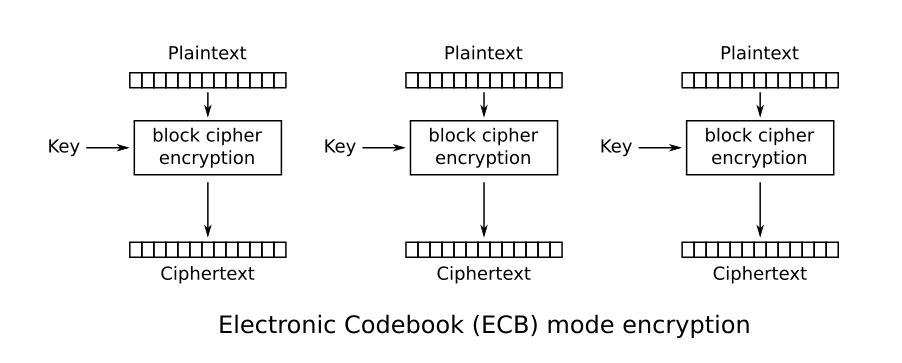
\includegraphics[width=\textwidth]{ECB_encryption.png}
    \caption{\acrlong{ecb} kryptering \cite{ecb-mode-enc-ref}}
    \label{fig:ecb-mode-enc}
\end{figure}

Figur \ref{fig:ecb-mode-dec} visar istället hur \acrshort{ecb} fungerar vid
dekryptering, vilken är en till stort sett identisk operation med det enda undantaget
att blockchiffret körs i dekrypterings läge istället för krypterings läge. % May need reformulating!!

\begin{figure}[H]
    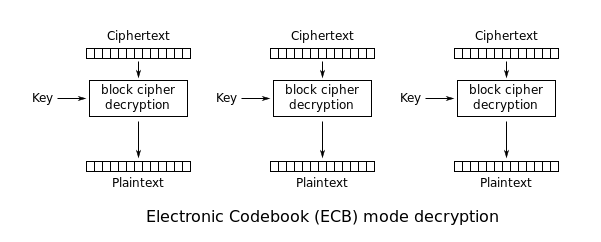
\includegraphics[width=\textwidth]{ECB_decryption.png}
    \caption{\acrlong{ecb} dekryptering \cite{ecb-mode-dec-ref}}
    \label{fig:ecb-mode-dec}
\end{figure}

På grund av \acrshort{ecb} körlägets simplicitet så finns det dock även ett ganska
stort problem med detta körläge. Det handlar om att \acrshort{ecb} inte på något
sätt förhindrar att två block med samma innehåll som krypteras inte resulterar i
ett identiskt krypterat block.\footcite{modesofoperation}

Vad detta innebär är att för större mängder data
är att det börjar bildas mönster i skiffertexten. Detta är något som väldigt
tydligt visar sig ifall man krypterar en bild, vilket går att se när man jämför
figur \ref{fig:pi-original} \& \ref{fig:pi-ecb}.
Det här faktumet är även varför \acrshort{ecb} inte är ett säkert körläge
och därför inte används näst intill aldrig i praktiken.\footcite{modesofoperation}

\acrshort{ecb} har däremot även sina fördelar då de bland annat kan parallelliseras
både när de gäller krypteringen och dekrypteringen. Detta samt att \acrshort{ecb}
även gör de möjligt att slumpmässigt dekryptera enskilda block av en skiffertext
utan att man behöver dekryptera hela texten.\footcite{modesofoperation}

\subsubsection{CBC}
\acrlong{cbc} är ett av de mest vanligen använda körlägena för många blockchiffer.
Till skillnad från \acrshort{ecb} så förhindrar \acrshort{cbc} att två block med
samma innehåll kan ge samma krypterade block. Detta gör \acrshort{cbc} genom att
lägga till ett extra steg utöver vad som finns i \acrshort{ecb}. Steget
är en \gls{xor}-operation mellan det krypterade blocket nästkommande block innan
de körs genom blockchiffer algoritmen.\footcite{modesofoperation}
Matematisk sett kan detta formuleras såhär:

\begin{equation}
    \label{eq:cbc-encryption}
    \begin{aligned}
        &S_i = K_n(B_i \oplus S_{i-1})\\\nonumber
        &S_0 = IV
    \end{aligned}
\end{equation}

Där $S_i$ är det krypterade blocket(skiffertexten), $B_i$ är det blocket som ska krypteras,
$K_n$ är blockchiffer algoritmen där $n$ står för nyckeln och $S_{i-1}$ är
det krypterade blocket före det blocket som ska krypteras. \acrshort{iv} är en
\acrfull{iv} som används vid krypteringen av de första blocket då de inte finns
något föregående block att använda. $i$ står för index där de första blocket har
index värdet 1. Hela den här processen kan även ses i figur \ref{fig:cbc-mode-enc}.

\begin{figure}[H]
    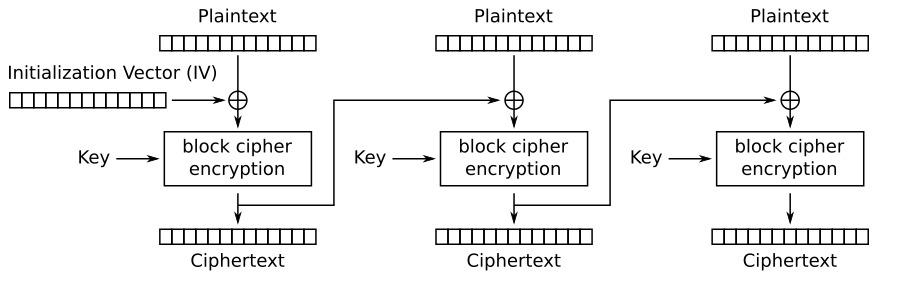
\includegraphics[width=\textwidth]{CBC_encryption.png}
    \caption{\acrlong{cbc} kryptering \cite{cbc-mode-enc-ref}}
    \label{fig:cbc-mode-enc}
\end{figure}

När de gäller dekrypterings processen för \acrshort{cbc} så bär den precis som för
\acrshort{ecb} stora likheter med krypterings processen. Det två skillnaderna som
finns är att blockchiffert körs i dekrypterings läge istället för krypterings läge.
Samt att för varje block så genomförs en \gls{xor}-operation mellan det dekrypterade
blocket och föregående block innan dekrypteringen av blocket.\footcite{modesofoperation}
Även detta går att både matematiskt formulera och visuellt visa såhär:

\begin{equation}
    \label{eq:cbc-decryption}
    \begin{aligned}
        &B_i = K_n(S_i) \oplus S_{i-1}\\\nonumber
        &S_0 = IV
    \end{aligned}
\end{equation}

\begin{figure}[H]
    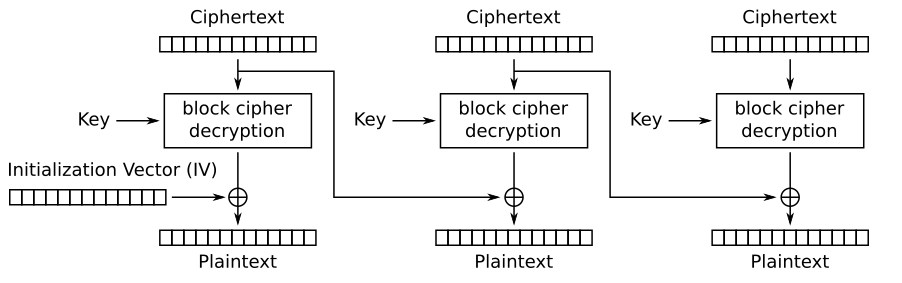
\includegraphics[width=\textwidth]{CBC_decryption.png}
    \caption{\acrlong{cbc} dekryptering \cite{cbc-mode-dec-ref}}
    \label{fig:cbc-mode-dec}
\end{figure}

Fördelarna som kommer från den extra operationen i \acrshort{cbc} till skillnad
från \acrshort{ecb} är då att varje block blir beroende av föregående block.
Detta innebär att dom mönster som kunde dyka upp i \acrshort{ecb} inte längre
kan uppstå, vilket då gör \acrshort{cbc} till ett mer säkert körläge än \acrshort{ecb}.
Dock kräver cbc en ytterligare faktor för att se till så att inte olika medelanden
kan ge samma krypterade block. Därav så krävs en \acrfull{iv} som används vid första
blocket.\footcite{modesofoperation}

\acrshort{cbc} är dock inte prefekt och har i sig också några nackdelar. Där ibland
exempelvis de faktum att en incorrect \acrshort{iv} leder till att de första blocket
inte kan dekrypteras korrekt, detta påverkar dock inte de resterande blocken. På grund
av det så kan man exempelvis lösa problemet genom att första blocket bara innehåller
någon typ av fyllnad, vilket då gör dekrypteringen möjlig utan tillgång till \acrshort{iv}.\footcite{modesofoperation}

Utöver detta så begränsas även \acrshort{cbc} till att bara vara parallelliserbar under
dekrypteringen och inte krypteringen, vilket är en konsekvens av att varje block i \acrshort{cbc}
är beroende av föregående block. \acrshort{cbc} behåller dock fortfarande möjligheten
som \acrshort{ecb} har att slumpmässigt dekryptera enskilda block utan att behöva
dekryptera hela skiffertexten.\footcite{modesofoperation}

\subsubsection{OFB}
\acrlong{ofb} är ett ytterligare körläge som skiljer sig en del från \acrshort{ecb}
och \acrshort{cbc} som  redan presenterats. Den största skillnaden från det andra
körlägena är att \acrshort{ofb} inte använder blockchiffer algoritmen för att kryptera
eller dekryptera blocken. Istället så körs \acrshort{iv} genom blockchiffer algoritmen
och den resulterande \gls{keystream} tillförs sedan genom en \gls{xor}-operation till
blocket som ska krypteras eller dekrypteras.\footcite{modesofoperation}

Tack vare \gls{xor}-operationens symmetriska natur så är så väl krypteringen som
dekrypteringen av \acrshort{ofb} identisk, vilket även visas i figur \ref{fig:ofb-mode-enc}
\& \ref{fig:ofb-mode-dec}:

\begin{figure}[H]
    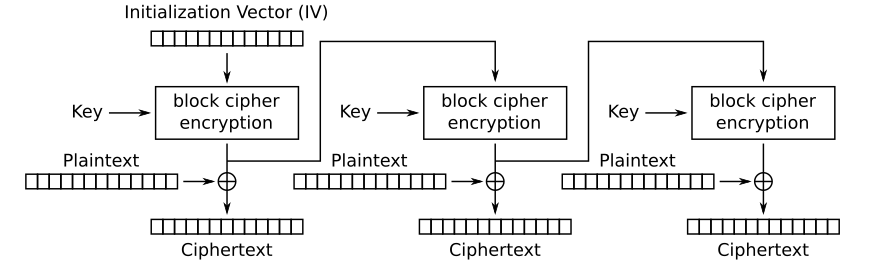
\includegraphics[width=\textwidth]{OFB_encryption.png}
    \caption{\acrlong{ofb} kryptering \cite{ofb-mode-enc-ref}}
    \label{fig:ofb-mode-enc}
\end{figure}

\begin{figure}[H]
    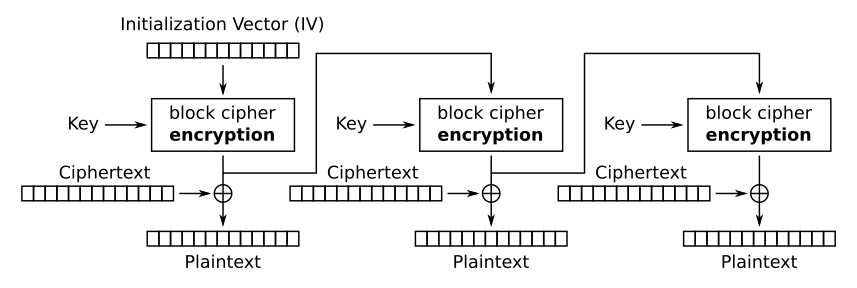
\includegraphics[width=\textwidth]{OFB_decryption.png}
    \caption{\acrlong{ofb} dekryptering \cite{ofb-mode-dec-ref}}
    \label{fig:ofb-mode-dec}
\end{figure}

Utöver detta kan man även matematiskt beskriva \acrshort{ofb}, vilket visas i ekvationen
nedan:

\begin{equation}
    \label{eq:ofb-encryption}
    \begin{aligned}
        &S_i = B_i \oplus O_i\\\nonumber
        &B_i = S_i \oplus O_i\\
        &O_i = K_n(I_i)\\
        &I_i = O_{i-1}\\
        &I_0 = IV
    \end{aligned}
\end{equation}

Här visas \acrshort{ofb} körläget matematiskt där $S_i$ är det krypterade blocket,
$B_i$ är blocket som ska krypteras och $I_0$ är \acrshort{iv}. Men här finns Även
$O_i$ som man kan säga är själva \gls{keystream} som används för att kryptera eller
dekryptera blocket. $O_i$ i sin tur bygger då på att $O_{i-1}$ körs genom blockchiffer
algoritmen igen och sedan används för nästa blocks kryptering.

På grund av att \acrshort{ofb} är utformat på det här sättet och att själva blocken som
ska krypteras inte används fram till sista steget så är det möjligt att genomföra blockskiffer
operationerna i förväg, vilket gör det möjligt att även parallellisera \acrshort{ofb}. Dock
kan \acrshort{ofb} inte parallelliseras ifall man inte gör blockskiffer operationerna
i förväg. Utöver detta saknar även \acrshort{ofb} möjligheten att slumpmässigt dekryptera
enskilda block utan att behöva dekryptera hela skiffertexten.\footcite{modesofoperation}

\section{Symetrisk \& Asymmetrisk Kryptering}
Symetrisk och asymetrisk kryptering handlar om hur nycklar används i olika
krypteringsalgoritmer. För symetriska krypterings algoritmer så betyder detta
att samma nyckel är vad som används för både kryptering och dekryptering. Medans
asymetrisk kryptering bygger på att man använder olika nycklar för kryptering och
dekrypterings processerna.\footfullcite{symencrypt}

De symetriska krypterings algoritmernas huvudsakliga nackdel ligger i de faktum att
de krävs en delad känd nyckel mellan båda parter. Detta är något som Asymetriska
krypterings algorithmer inte behöver, vilket har lett till att man ofta använder
asymetriska krypterings algoritmer för att sköta nyckelutbytet för de symetriska
krypterings algoritmerna. Anledningen till detta är att det symetriska krypterings
algoritmerna ofta är bättre för större data mängder då dom bland annat behöver mycket
kortare nyckellängder.\footcite{symencrypt}

Exempel på symetriska krypterings algoritmer är bland annat \acrshort{aes} och
\acrshort{des} var av \acrshort{aes} kommer förklaras djupare senare i denna rapport.\footcite{symencrypt}
Medans exempel på asymetriska krypterings algoritmer är bland annat \gls{rsa}.\footfullcite{rsa-ref}

\section{AES}


\subsection{Finite Fields}


\subsection{AES S-Box}


\subsection{Struktur}


\subsubsection{SubBytes operation}
SubBytes operationen bygger på ...

\subsubsection{ShiftRows operation}


\subsubsection{MixColumns operation}


\subsubsection{AddRoundKey operation}


\subsection{Nyckel utökning}


\subsubsection{RotWord}


\subsubsection{SubWord}


\subsubsection{Rcon}


\subsection{AES-128bit}


\subsection{AES-192bit}


\subsection{AES-256bit}



\include{Material_utförande}

\mychapter{Resultat}
\label{chap:resultat}
Notera att tiden som visas i tabellerna är i sekunder och är ett medelvärde av 25 enskilda
krypteringsomgångar för varje nyckel och varje körläge.
För att se tiderna för varje individuell omgång samt bilderna i större storlek
se bilaga \ref{app:raw-data-mode-picture-test}, \ref{app:raw-data-keylength} \& \ref{app:raw-data-mode}.

\section{Nyckellängdstest}
\label{sec:nyckellangd}

\begin{table}[H]
    \centering
    \begin{tabular}{ |c|c|c|c| }
      \multicolumn{4}{c}{\bfseries{Resultat Tid (s)}} \\
      \hline
      & \bfseries{ECB - 128bit} & \bfseries{ECB - 192bit} & \bfseries{ECB - 256bit} \\
      \hline
      \bfseries{Maxvärde} & 21,71 & 25,31 & 29,28 \\
      \hline
      \bfseries{Minvärde} & 20,84 & 24,89 & 29,03 \\
      \hline
      \bfseries{Medelvärde} & 21,06 & 25,01 & 29,18 \\
      \hline
    \end{tabular}
\end{table}

\begin{table}[H]
  \centering
  \begin{tabular}{ |c|c| }
    \multicolumn{2}{c}{\bfseries{Procentuell skillnad (medelvärde)}} \\
    \hline
    \bfseries{ECB - 128bit \& 192bit} & 18,8\% \\
    \hline
    \bfseries{ECB - 192bit \& 256bit} & 16,6\% \\
    \hline
    \bfseries{ECB - 128bit \& 256bit} & 27,8\% \\
    \hline
  \end{tabular}
\end{table}

\section{Körlägestest}
\label{sec:korlages}

\begin{table}[H]
    \centering
    \begin{tabular}{ |c|c|c|c| }
      \multicolumn{4}{c}{\bfseries{Resultat Tid (s)}} \\
      \hline
      & \bfseries{ECB - 128bit} & \bfseries{CBC - 128bit} & \bfseries{OFB - 128bit} \\
      \hline
      \bfseries{Maxvärde} & 21,09 & 20,93 & 20,88 \\
      \hline
      \bfseries{Minvärde} & 20,80 & 20,85 & 20,77 \\
      \hline
      \bfseries{Medelvärde} & 20.82 & 20.89 & 20.90 \\
      \hline
    \end{tabular}
\end{table}

\begin{table}[H]
  \centering
  \begin{tabular}{ |c|c| }
    \multicolumn{2}{c}{\bfseries{Procentuell skillnad (medelvärde)}} \\
    \hline
    \bfseries{ECB - 128bit \& CBC - 128bit} & 0,3\% \\
    \hline
    \bfseries{CBC - 128bit \& OFB - 128bit} & 0,1\% \\
    \hline
    \bfseries{ECB - 128bit \& OFB - 128bit} & 0,4\% \\
    \hline
  \end{tabular}
\end{table}

\section{Krypteringstest}
\label{sec:krypterings-test}

\begin{figure}[H]
      \centering
    \includegraphics[width=0.8\textwidth]{summarie-tp-background.png}
    \caption{\acrshort{aes} krypterings test (\acrshort{ecb}, \acrshort{cbc}, \acrshort{ofb})}
    \label{fig:aes-krypterings-test}
\end{figure}


\mychapter{Diskussion \& Slutord} % Diskussion av resultat, presentera och tolka resultatet samt för ett nyanserat resonemang om vad resultatet betyder. Diskutera även eventuella brister i experimentet och hur dessa kan förbättras.
\label{chap:discussion}

Utifrån resultatet från undersökningen kan man då se hur tiden det tar att kryptera en fil på 1MB ökar när man använder längre nycklar så som 192-\gls{bit} 256-\gls{bit} nycklar.
Samtidigt visar det sig även att skillnaden i krypteringstid mellan olika körlägen är väldigt liten. Något som tydligt visas det procentuella tids skillnaderna där
det som högst skiljde sig med 0,4\% mellan \acrshort{ecb} \& \acrshort{ofb}. Medans skillnaden mellan \acrshort{cbc} \& \acrshort{ofb} var 0,1\%.

Tittar man sedan istället på hur säkerheten påverkas av det olika körlägena så kan man ganska tydligt se att \acrshort{ecb} är det mest osäkra körläget för större data mängder.
Detta då man som visas i resultatet kan se hur trots kryptering man fortfarande kan se spår av den ursprungliga bilden i informationen som krypterats. Något som inte
går att göra när bilden istället krypteras med hjälp av \acrshort{cbc} eller \acrshort{ofb}.


\section{Felkällor} % Variabilitet i klockhastighet, Ogämnheter i implementeringen som resutlerar i missvisande tider, osäkerhet host mätmetoden, fel i implementeringen, 


\section{Förbättringar} % Öka antalet reppetitioner för att minskar risken för fel, använda andra metoder för att mäta tiden, testa olika nycklar för att se hur de påverkar, 


\section{Slutsats}


\section{Slutord}


\fakechapter{Källförteckning}{7}
\addcontentsline{toc}{chapter}{Källförteckning}
\printbibliography[title=Källförteckning]

\clearpage

\appendix

\chapter{AES körläges test resultat}
\label{app:raw-data-mode-picture-test}

\section{Före testet}
\begin{figure}[H]
  \centering
  
\includegraphics[width=0.6\textwidth]{pi.png}
  \caption{Orginal bild}
  \label{fig:pi-original}
\end{figure}

\section{Efter ECB kryptering}
\begin{figure}[H]
  \centering
  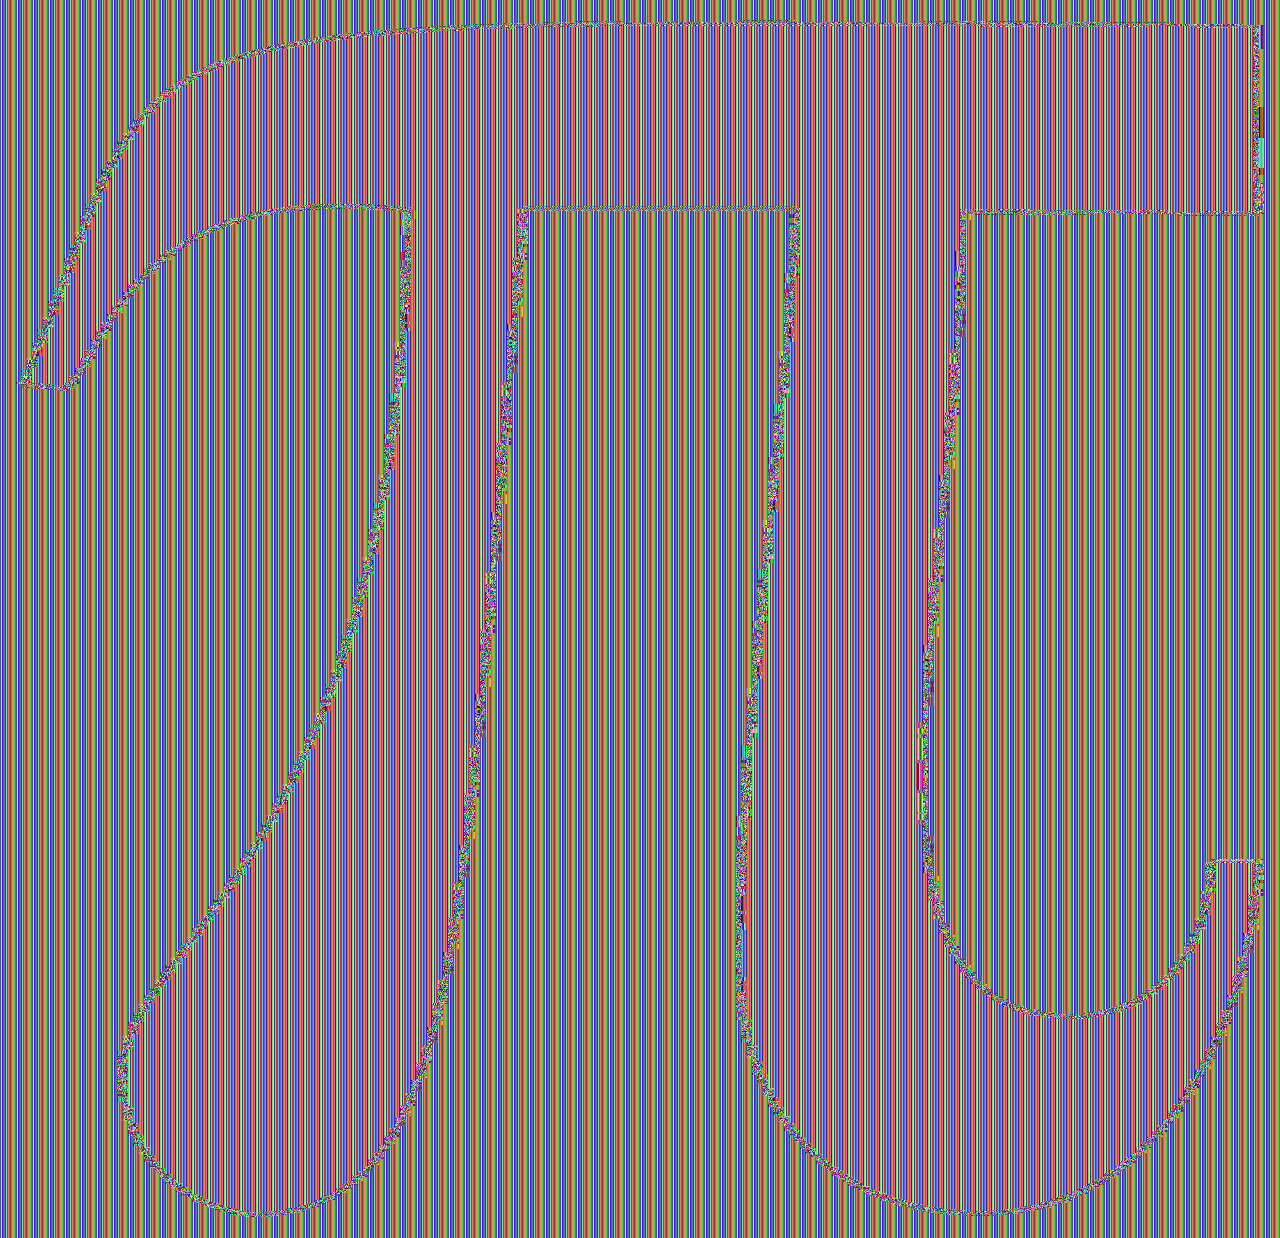
\includegraphics[width=0.6\textwidth]{pi-ecb.png}
  \caption{Efter ECB Kryptering}
  \label{fig:pi-ecb}
\end{figure}

\section{Efter CBC kryptering}
\begin{figure}[H]
  \centering
  \includegraphics[width=0.6\textwidth]{pi-cbc.png}
  \caption{Efter CBC Kryptering}
  \label{fig:pi-cbc}
\end{figure}

\section{Efter CFB kryptering}
\begin{figure}[H]
  \centering
  \includegraphics[width=0.6\textwidth]{pi-OFB.png}
  \caption{Efter OFB Kryptering}
  \label{fig:pi-ofb}
\end{figure}

\cleardoublepage

\chapter{Rå data från test}
\label{app:raw-data}

\section{Data från Nyckellängds test}
\label{app:raw-data-keylength}

\begin{table}[H]
    \centering
    \begin{tabular}{ ||c|c|c|| }
      \hline
      \multicolumn{3}{|c|}{\bfseries{Resultat Tid (s)}} \\
      \hline
      \bfseries{ECB - 128bit} & \bfseries{ECB - 192bit} & \bfseries{ECB - 256bit} \\
      \hline
      21.114332500001183 & 25.019810000005236 & 29.25573820000136 \\
      21.2294222000055 & 25.03902250000101 & 29.199436000002606 \\
      21.400101300001552 & 24.921688300004462 & 29.1446350000042 \\
      21.394803399998636 & 25.010479399999895 & 29.276371100000688 \\
      21.410092899997835 & 25.023025200003758 & 29.208361999997578 \\
      21.255479499996 & 24.94711079999979 & 29.12308629999461 \\
      21.709606899996288 & 24.932161500000802 & 29.057567500000005 \\
      20.930029600000125 & 24.93615460000001 & 29.23549970000022 \\
      20.91164679999929 & 25.07268920000206 & 29.163480200004415 \\
      21.024735999999393 & 25.05104990000109 & 29.13999270000204 \\
      20.974247600002855 & 24.92792770000233 & 29.03159289999894 \\
      20.906690399999206 & 25.040346800000407 & 29.238432199999806 \\
      20.949946799999452 & 25.02671339999506 & 29.226332500002172 \\
      20.96879309999349 & 24.999294099994586 & 29.13317239999742 \\
      20.955687699999544 & 24.973698000001605 & 29.119369399995776 \\
      20.907472200000484 & 24.992430599995714 & 29.273320899999817 \\
      20.99763510000048 & 25.22444600000017 & 29.147454799996922 \\
      20.964201399998274 & 25.310352100001182 & 29.133893199999875 \\
      20.970198600000003 & 25.03863189999538 & 29.14858010000171 \\
      21.033452000003308 & 24.887886799995613 & 29.20511969999643 \\
      20.835713899999973 & 25.002411200002825 & 29.214967400002934 \\
      20.933525599997665 & 25.029954099998577 & 29.155635700000857 \\
      20.899700900001335 & 24.92795739999565 & 29.136839000006148 \\
      20.861958300003607 & 25.015061800004332 & 29.250083099999756 \\
      20.898621000000276 & 25.012236000002304 & 29.22063089999574 \\
      \hline
    \end{tabular}
  \end{table}

\section{Data från körläges test}
\label{app:raw-data-mode}

\begin{table}[H]
    \centering
    \begin{tabular}{ ||c|c|c|| }
      \hline
      \multicolumn{3}{|c|}{\bfseries{Resultat Tid (s)}} \\
      \hline
      \bfseries{ECB} & \bfseries{CBC} & \bfseries{OFB} \\
      \hline
      20.855055499996524 & 20.863876399998844 & 20.801168300000427 \\
      20.88846609999746 & 20.907602499995846 & 20.78754040000058 \\
      20.879108299996005 & 20.86540999999852 & 20.823867599996447 \\
      20.801008999995247 & 20.896374500000093 & 20.87718119999772 \\
      20.85887470000307 & 20.868871400001808 & 20.770114799997828 \\
      20.87116899999819 & 20.882914800000435 & 20.767576799997187 \\
      20.854077200005122 & 20.89511720000155 & 20.85902029999852 \\
      20.85488130000158 & 20.85610540000198 & 20.797623000005842 \\
      20.826587200004724 & 20.865844100000686 & 20.796596600004705 \\
      20.909639099998458 & 20.85497480000049 & 20.797125700002653 \\
      20.870294899999863 & 20.906652400000894 & 20.835499799999525 \\
      20.818692400003783 & 20.92016809999768 & 20.865253799995116 \\
      20.82849349999742 & 20.908798900003603 & 20.800847200000135 \\
      20.86879109999427 & 20.850567699999374 & 20.795617399999173 \\
      20.91046159999678 & 20.883563499999582 & 20.834485100000165 \\
      20.82723100000294 & 20.884897599993565 & 20.82335030000104 \\
      20.80391700000473 & 20.89037549999921 & 20.828929399998742 \\
      20.87521669999842 & 20.885131600000022 & 20.811529400001746 \\
      20.91481080000085 & 20.93468269999721 & 20.881663000000117 \\
      21.085760299996764 & 20.859826599997177 & 20.85081160000118 \\
      20.97296980000101 & 20.875606900001003 & 20.823041400006332 \\
      21.053496200001973 & 20.903108300000895 & 20.791531299997587 \\
      20.978821899996547 & 20.892179500006023 & 20.878361099996255 \\
      20.954259099999035 & 20.890548900002614 & 20.873186500000884 \\
      21.028453000006266 & 20.88354160000017 & 20.76938550000341 \\
      \hline
    \end{tabular}
  \end{table}

\chapter{AES Implementering i python}
\label{app:python}

\section{AES.py}

\begin{python}
# ---------------
# Imported libraries
# ---------------
from os.path import getsize
from os import remove
import numpy as np

# ---------------
# Fixed variables
# ---------------
# Sbox & inverse Sbox
subBytesTable = (
    0x63, 0x7c, 0x77, 0x7b, 0xf2, 0x6b, 0x6f, 0xc5, 0x30, 0x01, 0x67, 0x2b, 0xfe, 0xd7, 0xab, 0x76,
    0xca, 0x82, 0xc9, 0x7d, 0xfa, 0x59, 0x47, 0xf0, 0xad, 0xd4, 0xa2, 0xaf, 0x9c, 0xa4, 0x72, 0xc0,
    0xb7, 0xfd, 0x93, 0x26, 0x36, 0x3f, 0xf7, 0xcc, 0x34, 0xa5, 0xe5, 0xf1, 0x71, 0xd8, 0x31, 0x15,
    0x04, 0xc7, 0x23, 0xc3, 0x18, 0x96, 0x05, 0x9a, 0x07, 0x12, 0x80, 0xe2, 0xeb, 0x27, 0xb2, 0x75,
    0x09, 0x83, 0x2c, 0x1a, 0x1b, 0x6e, 0x5a, 0xa0, 0x52, 0x3b, 0xd6, 0xb3, 0x29, 0xe3, 0x2f, 0x84,
    0x53, 0xd1, 0x00, 0xed, 0x20, 0xfc, 0xb1, 0x5b, 0x6a, 0xcb, 0xbe, 0x39, 0x4a, 0x4c, 0x58, 0xcf,
    0xd0, 0xef, 0xaa, 0xfb, 0x43, 0x4d, 0x33, 0x85, 0x45, 0xf9, 0x02, 0x7f, 0x50, 0x3c, 0x9f, 0xa8,
    0x51, 0xa3, 0x40, 0x8f, 0x92, 0x9d, 0x38, 0xf5, 0xbc, 0xb6, 0xda, 0x21, 0x10, 0xff, 0xf3, 0xd2,
    0xcd, 0x0c, 0x13, 0xec, 0x5f, 0x97, 0x44, 0x17, 0xc4, 0xa7, 0x7e, 0x3d, 0x64, 0x5d, 0x19, 0x73,
    0x60, 0x81, 0x4f, 0xdc, 0x22, 0x2a, 0x90, 0x88, 0x46, 0xee, 0xb8, 0x14, 0xde, 0x5e, 0x0b, 0xdb,
    0xe0, 0x32, 0x3a, 0x0a, 0x49, 0x06, 0x24, 0x5c, 0xc2, 0xd3, 0xac, 0x62, 0x91, 0x95, 0xe4, 0x79,
    0xe7, 0xc8, 0x37, 0x6d, 0x8d, 0xd5, 0x4e, 0xa9, 0x6c, 0x56, 0xf4, 0xea, 0x65, 0x7a, 0xae, 0x08,
    0xba, 0x78, 0x25, 0x2e, 0x1c, 0xa6, 0xb4, 0xc6, 0xe8, 0xdd, 0x74, 0x1f, 0x4b, 0xbd, 0x8b, 0x8a,
    0x70, 0x3e, 0xb5, 0x66, 0x48, 0x03, 0xf6, 0x0e, 0x61, 0x35, 0x57, 0xb9, 0x86, 0xc1, 0x1d, 0x9e,
    0xe1, 0xf8, 0x98, 0x11, 0x69, 0xd9, 0x8e, 0x94, 0x9b, 0x1e, 0x87, 0xe9, 0xce, 0x55, 0x28, 0xdf,
    0x8c, 0xa1, 0x89, 0x0d, 0xbf, 0xe6, 0x42, 0x68, 0x41, 0x99, 0x2d, 0x0f, 0xb0, 0x54, 0xbb, 0x16
    )

invSubBytesTable = (
    0x52, 0x09,	0x6a, 0xd5, 0x30, 0x36,	0xa5, 0x38,	0xbf, 0x40,	0xa3, 0x9e, 0x81, 0xf3, 0xd7, 0xfb,
    0x7c, 0xe3,	0x39, 0x82, 0x9b, 0x2f,	0xff, 0x87,	0x34, 0x8e,	0x43, 0x44, 0xc4, 0xde, 0xe9, 0xcb,
    0x54, 0x7b,	0x94, 0x32, 0xa6, 0xc2,	0x23, 0x3d,	0xee, 0x4c,	0x95, 0x0b, 0x42, 0xfa, 0xc3, 0x4e,
    0x08, 0x2e,	0xa1, 0x66, 0x28, 0xd9,	0x24, 0xb2,	0x76, 0x5b,	0xa2, 0x49, 0x6d, 0x8b, 0xd1, 0x25,
    0x72, 0xf8,	0xf6, 0x64, 0x86, 0x68,	0x98, 0x16,	0xd4, 0xa4,	0x5c, 0xcc, 0x5d, 0x65, 0xb6, 0x92,
    0x6c, 0x70,	0x48, 0x50, 0xfd, 0xed,	0xb9, 0xda,	0x5e, 0x15,	0x46, 0x57, 0xa7, 0x8d, 0x9d, 0x84,
    0x90, 0xd8,	0xab, 0x00, 0x8c, 0xbc,	0xd3, 0x0a,	0xf7, 0xe4,	0x58, 0x05, 0xb8, 0xb3, 0x45, 0x06,
    0xd0, 0x2c,	0x1e, 0x8f, 0xca, 0x3f,	0x0f, 0x02,	0xc1, 0xaf,	0xbd, 0x03, 0x01, 0x13, 0x8a, 0x6b,
    0x3a, 0x91,	0x11, 0x41, 0x4f, 0x67,	0xdc, 0xea,	0x97, 0xf2,	0xcf, 0xce, 0xf0, 0xb4, 0xe6, 0x73,
    0x96, 0xac,	0x74, 0x22, 0xe7, 0xad,	0x35, 0x85,	0xe2, 0xf9,	0x37, 0xe8, 0x1c, 0x75, 0xdf, 0x6e,
    0x47, 0xf1,	0x1a, 0x71, 0x1d, 0x29,	0xc5, 0x89,	0x6f, 0xb7,	0x62, 0x0e, 0xaa, 0x18, 0xbe, 0x1b,
    0xfc, 0x56,	0x3e, 0x4b, 0xc6, 0xd2,	0x79, 0x20,	0x9a, 0xdb,	0xc0, 0xfe, 0x78, 0xcd, 0x5a, 0xf4,
    0x1f, 0xdd,	0xa8, 0x33, 0x88, 0x07,	0xc7, 0x31,	0xb1, 0x12,	0x10, 0x59, 0x27, 0x80, 0xec, 0x5f,
    0x60, 0x51,	0x7f, 0xa9, 0x19, 0xb5,	0x4a, 0x0d,	0x2d, 0xe5,	0x7a, 0x9f, 0x93, 0xc9, 0x9c, 0xef,
    0xa0, 0xe0,	0x3b, 0x4d, 0xae, 0x2a,	0xf5, 0xb0,	0xc8, 0xeb,	0xbb, 0x3c, 0x83, 0x53, 0x99, 0x61,
    0x17, 0x2b,	0x04, 0x7e, 0xba, 0x77,	0xd6, 0x26,	0xe1, 0x69,	0x14, 0x63, 0x55, 0x21, 0x0c, 0x7d
    )

# Round constants
round_constant = (
    0x00000000, 0x01000000, 0x02000000,
    0x04000000, 0x08000000, 0x10000000,
    0x20000000, 0x40000000, 0x80000000,
    0x1B000000, 0x36000000, 0x6C000000,
    0xD8000000, 0xAB000000, 0x4D000000,
    )


# ---------------
# Main action functions
# ---------------
# Xtime
def xtime(a):
    return (((a << 1) ^ 0x1B) & 0xFF) if (a & 0x80) else (a << 1)


# Performs the byte substitution layer
def sub_bytes(data, bytesTable):
    for i, row in enumerate(data):
        for j, byte in enumerate(row):
            data[i][j] = bytesTable[byte]
    return data


# Shift rows function
def shift_rows(array):
    array[:, 1] = np.roll(array[:, 1], -1, axis=0)
    array[:, 2] = np.roll(array[:, 2], -2, axis=0)
    array[:, 3] = np.roll(array[:, 3], -3, axis=0)
    return array


# Inverse shift rows function
def inv_shift_rows(array):
    array[:, 1] = np.roll(array[:, 1], 1, axis=0)
    array[:, 2] = np.roll(array[:, 2], 2, axis=0)
    array[:, 3] = np.roll(array[:, 3], 3, axis=0)
    return array


# Performs the mix columns layer
def mix_columns(data):
    def mix_single_column(data):
        # See Sec 4.1.2 in The Design of Rijndael
        t = data[0] ^ data[1] ^ data[2] ^ data[3]
        u = data[0]
        data[0] ^= t ^ xtime(data[0] ^ data[1])
        data[1] ^= t ^ xtime(data[1] ^ data[2])
        data[2] ^= t ^ xtime(data[2] ^ data[3])
        data[3] ^= t ^ xtime(data[3] ^ u)

    def mix(data):
        for i in range(4):
            mix_single_column(data[i])
        return data
    data = mix(data)
    return data


# Preforms the inverse mix columns layer
def inv_mix_columns(data):
    # See Sec 4.1.3 in The Design of Rijndael
    for i in range(4):
        u = xtime(xtime(data[i][0] ^ data[i][2]))
        v = xtime(xtime(data[i][1] ^ data[i][3]))
        data[i][0] ^= u
        data[i][1] ^= v
        data[i][2] ^= u
        data[i][3] ^= v
    mix_columns(data)
    return data


# Adds a padding to ensure a bloke size of 16 bytes
def add_padding(data):
    length = 16 - len(data)
    for i in range(length):
        data.append(0)
    return data, length


# Removes the padding
def remove_padding(data, identifier):
    if identifier[-1] == 0:
        return data
    elif identifier[-1] > 0 and identifier[-1] < 16:
        return data[:-identifier[-1]]
    else:
        raise ValueError('Invalid padding')


# Performs the encryption rounds
def encryption_rounds(data, round_keys, nr):
    # Inizial add round key
    data = np.bitwise_xor(data, round_keys[0])

    # Rounds 1 to 9 or 1 to 11 or 1 to 13
    for i in range(1, (nr - 1)):
        data = sub_bytes(data, subBytesTable)
        data = shift_rows(data)
        data = mix_columns(data)
        data = np.bitwise_xor(data, round_keys[i])

    # Final round
    data = sub_bytes(data, subBytesTable)
    data = shift_rows(data)
    data = np.bitwise_xor(data, round_keys[nr - 1])

    return data


# Performs the decryption rounds
def decryption_rounds(data, round_keys, nr):
    # Inizial add round key
    data = np.bitwise_xor(data, round_keys[-1])

    # Rounds 1 to 9 or 1 to 11 or 1 to 13
    for i in range(1, (nr - 1)):
        data = inv_shift_rows(data)
        data = sub_bytes(data, invSubBytesTable)
        data = np.bitwise_xor(data, round_keys[-(i+1)])
        data = inv_mix_columns(data)

    # Final round
    data = inv_shift_rows(data)
    data = sub_bytes(data, invSubBytesTable)
    data = np.bitwise_xor(data, round_keys[0])

    return data


# ---------------
# Key expansion setup
# ---------------
# Key expansion function (returns a list of round keys)
def keyExpansion(key):
    # Format key correctly for the key expansion
    key = [key[i:i+2] for i in range(0, len(key), 2)]

    # Key expansion setup
    if len(key) == 16:
        words = key_schedule(key, 4, 11)
        nr = 11
    if len(key) == 24:
        words = key_schedule(key, 6, 13)
        nr = 13
    if len(key) == 32:
        words = key_schedule(key, 8, 15)
        nr = 15

    round_keys = [None for i in range(nr)]

    tmp = [None for i in range(4)]

    for i in range(nr * 4):
        for index, t in enumerate(words[i]):
            tmp[index] = int(t, 16)  # type: ignore
        words[i] = tuple(tmp)

    for i in range(nr):
        round_keys[i] = np.array(words[i * 4] + words[i * 4 + 1] + words[i * 4 + 2] + words[i * 4 + 3]).reshape(4, 4)  # type: ignore

    return round_keys, nr


# Key schedule (nk = number of colums, nr = number of rounds)
def key_schedule(key, nk, nr):
    # Create list and populates first nk words with key
    words = [(key[4*i], key[4*i+1], key[4*i+2], key[4*i+3]) for i in range(nk)]

    # Fill out the rest based on previews words, rotword, subword and rcon values
    limit = False
    for i in range(nk, (nr * nk)):
        # Get required previous keywords
        temp, word = words[i-1], words[i-nk]

        # If multiple of nk use rot, sub, rcon etc
        if i % nk == 0:
            x = SubWord(RotWord(temp))
            rcon = round_constant[int(i/nk)]
            temp = hexor(x, hex(rcon)[2:])
            limit = False
        elif i % 4 == 0:
            limit = True

        if i % 4 == 0 and limit and nk >= 8:
            temp = SubWord(temp)

        # Xor the two hex values
        xord = hexor(''.join(word), ''.join(temp))
        words.append((xord[:2], xord[2:4], xord[4:6], xord[6:8]))
    return words


# Takes two hex values and calculates hex1 xor hex2
def hexor(hex1, hex2):
    # Convert to binary
    bin1 = hex2binary(hex1)
    bin2 = hex2binary(hex2)

    # Calculate
    xord = int(bin1, 2) ^ int(bin2, 2)

    # Cut prefix
    hexed = hex(xord)[2:]

    # Leading 0s get cut above, if not length 8 add a leading 0
    if len(hexed) != 8:
        hexed = '0' + hexed

    return hexed


# Takes a hex value and returns binary
def hex2binary(hex):
    return bin(int(str(hex), 16))


# Takes from 1 to the end, adds on from the start to 1
def RotWord(word):
    return word[1:] + word[:1]


# Selects correct value from sbox based on the current word
def SubWord(word):
    sWord = []

    # Loop throug the current word
    for i in range(4):

        # Check first char, if its a letter(a-f) get corresponding decimal
        # otherwise just take the value and add 1
        if word[i][0].isdigit() is False:
            row = ord(word[i][0]) - 86
        else:
            row = int(word[i][0])+1

        # Repeat above for the seoncd char
        if word[i][1].isdigit() is False:
            col = ord(word[i][1]) - 86
        else:
            col = int(word[i][1])+1

        # Get the index base on row and col (16x16 grid)
        sBoxIndex = (row*16) - (17-col)

        # Get the value from sbox without prefix
        piece = hex(subBytesTable[sBoxIndex])[2:]

        # Check length to ensure leading 0s are not forgotton
        if len(piece) != 2:
            piece = '0' + piece

        sWord.append(piece)

    # Return string
    return ''.join(sWord)


# ---------------
# Running modes setup
# ---------------
# ECB encryption function
def ecb_enc(key, file_path):
    file_size = getsize(file_path)
    round_keys, nr = keyExpansion(key)

    with open(f"{file_path}.enc", 'wb') as output, open(file_path, 'rb') as data:
        for i in range(int(file_size/16)):
            raw = np.array([i for i in data.read(16)]).reshape(4, 4)
            result = bytes((encryption_rounds(raw, round_keys, nr).flatten()).tolist())
            output.write(result)

        if file_size % 16 != 0:
            raw = [i for i in data.read()]  # type: ignore
            raw, length = add_padding(raw)

            result = bytes((encryption_rounds(np.array(raw).reshape(4, 4), round_keys, nr).flatten()).tolist())
            identifier = bytes((encryption_rounds(np.array([0 for i in range(15)] + [length]).reshape(4, 4), round_keys, nr).flatten()).tolist())

            output.write(result + identifier)
        else:
            identifier = bytes((encryption_rounds(np.array([0 for i in range(16)]).reshape(4, 4), round_keys, nr).flatten()).tolist())
            output.write(identifier)
    remove(file_path)


# ECB decryption function
def ecb_dec(key, file_path):
    file_size = getsize(file_path)
    file_name = file_path[:-4]
    round_keys, nr = keyExpansion(key)

    with open(f"{file_name}", 'wb') as output, open(file_path, 'rb') as data:
        for i in range(int(file_size/16) - 2):
            raw = np.array([i for i in data.read(16)]).reshape(4, 4)
            result = bytes((decryption_rounds(raw, round_keys, nr).flatten()).tolist())
            output.write(result)

        data_pice = np.array([i for i in data.read(16)]).reshape(4, 4)
        identifier = np.array([i for i in data.read()]).reshape(4, 4)

        result = (decryption_rounds(data_pice, round_keys, nr).flatten()).tolist()
        identifier = (decryption_rounds(identifier, round_keys, nr).flatten()).tolist()

        result = bytes(remove_padding(result, identifier))

        output.write(result)
    remove(file_path)


# CBC encryption function
def cbc_enc(key, file_path, iv):
    file_size = getsize(file_path)
    vector = np.array([int(iv[i:i+2], 16) for i in range(0, len(iv), 2)]).reshape(4, 4)
    round_keys, nr = keyExpansion(key)

    with open(f"{file_path}.enc", 'wb') as output, open(file_path, 'rb') as data:
        for i in range(int(file_size/16)):
            raw = np.array([i for i in data.read(16)]).reshape(4, 4)
            raw = np.bitwise_xor(raw, vector)
            vector = encryption_rounds(raw, round_keys, nr)
            output.write(bytes((vector.flatten()).tolist()))

        if file_size % 16 != 0:
            raw = [i for i in data.read()]  # type: ignore
            raw, length = add_padding(raw)

            raw = np.bitwise_xor(np.array(raw).reshape(4, 4), vector)
            vector = encryption_rounds(raw, round_keys, nr)

            identifier = np.bitwise_xor(np.array([0 for i in range(15)] + [length]).reshape(4, 4), vector)
            identifier = encryption_rounds(identifier, round_keys, nr)

            output.write(bytes((vector.flatten()).tolist() + (identifier.flatten()).tolist()))
        else:
            identifier = np.bitwise_xor(np.array([0 for i in range(16)]).reshape(4, 4), vector)
            identifier = bytes(((encryption_rounds(identifier, round_keys, nr)).flatten()).tolist())  # type: ignore
            output.write(identifier)  # type: ignore
    remove(file_path)


# CBC decryption function
def cbc_dec(key, file_path, iv):
    iv = np.array([int(iv[i:i+2], 16) for i in range(0, len(iv), 2)]).reshape(4, 4)
    file_size = getsize(file_path)
    file_name = file_path[:-4]
    round_keys, nr = keyExpansion(key)

    with open(f"{file_name}", 'wb') as output, open(file_path, 'rb') as data:
        if int(file_size/16) - 3 >= 0:
            vector = np.array([i for i in data.read(16)]).reshape(4, 4)
            raw = decryption_rounds(vector, round_keys, nr)
            result = np.bitwise_xor(raw, iv)
            output.write(bytes((result.flatten()).tolist()))

            for i in range(int(file_size/16) - 3):
                raw = np.array([i for i in data.read(16)]).reshape(4, 4)
                result = decryption_rounds(raw, round_keys, nr)
                result = np.bitwise_xor(result, vector)
                vector = raw
                output.write(bytes((result.flatten()).tolist()))
        else:
            vector = iv

        data_pice = np.array([i for i in data.read(16)]).reshape(4, 4)
        vector_1, identifier = data_pice, np.array([i for i in data.read()]).reshape(4, 4)

        result = decryption_rounds(data_pice, round_keys, nr)
        identifier = decryption_rounds(identifier, round_keys, nr)

        identifier = np.bitwise_xor(identifier, vector_1)
        data_pice = np.bitwise_xor(result, vector)

        result = bytes(remove_padding((data_pice.flatten()).tolist(), (identifier.flatten()).tolist()))

        output.write(result)
    remove(file_path)


# PCBC encryption function
def pcbc_enc(key, file_path, iv):
    file_size = getsize(file_path)
    vector = np.array([int(iv[i:i+2], 16) for i in range(0, len(iv), 2)]).reshape(4, 4)
    round_keys, nr = keyExpansion(key)

    with open(f"{file_path}.enc", 'wb') as output, open(file_path, 'rb') as data:
        for i in range(int(file_size/16)):
            raw = np.array([i for i in data.read(16)]).reshape(4, 4)
            tmp = np.bitwise_xor(raw, vector)
            vector = encryption_rounds(tmp, round_keys, nr)
            output.write(bytes((vector.flatten()).tolist()))
            vector = np.bitwise_xor(vector, raw)

        if file_size % 16 != 0:
            raw = [i for i in data.read()]  # type: ignore
            raw, length = add_padding(raw)
            raw = np.array(raw).reshape(4, 4)

            tmp = np.bitwise_xor(raw, vector)
            vector1 = encryption_rounds(tmp, round_keys, nr)
            vector = np.bitwise_xor(vector1, raw)

            identifier = np.bitwise_xor(np.array([0 for i in range(15)] + [length]).reshape(4, 4), vector)
            identifier = encryption_rounds(identifier, round_keys, nr)

            output.write(bytes((vector1.flatten()).tolist() + (identifier.flatten()).tolist()))
        else:
            identifier = np.bitwise_xor(np.array([0 for i in range(16)]).reshape(4, 4), vector)
            identifier = bytes((encryption_rounds(identifier, round_keys, nr).flatten()).tolist())  # type: ignore
            output.write(identifier)  # type: ignore
    remove(file_path)


# PCBC decryption function
def pcbc_dec(key, file_path, iv):
    iv = np.array([int(iv[i:i+2], 16) for i in range(0, len(iv), 2)]).reshape(4, 4)
    file_size = getsize(file_path)
    file_name = file_path[:-4]
    round_keys, nr = keyExpansion(key)

    with open(f"{file_name}", 'wb') as output, open(file_path, 'rb') as data:
        if int(file_size/16) - 3 >= 0:
            vector = np.array([i for i in data.read(16)]).reshape(4, 4)
            raw = decryption_rounds(vector, round_keys, nr)
            result = np.bitwise_xor(raw, iv)
            vector = np.bitwise_xor(vector, result)
            output.write(bytes((result.flatten()).tolist()))

            for i in range(int(file_size/16) - 3):
                raw = np.array([i for i in data.read(16)]).reshape(4, 4)
                result = decryption_rounds(raw, round_keys, nr)
                result = np.bitwise_xor(result, vector)
                vector = np.bitwise_xor(raw, result)
                output.write(bytes((result.flatten()).tolist()))
        else:
            vector = iv

        data_pice = np.array([i for i in data.read(16)]).reshape(4, 4)
        vector_1, identifier = data_pice, np.array([i for i in data.read()]).reshape(4, 4)

        result = decryption_rounds(data_pice, round_keys, nr)
        data_pice = np.bitwise_xor(result, vector)

        vector_1 = np.bitwise_xor(vector_1, data_pice)
        identifier = decryption_rounds(identifier, round_keys, nr)
        identifier = np.bitwise_xor(identifier, vector_1)

        result = bytes(remove_padding((data_pice.flatten()).tolist(), (identifier.flatten()).tolist()))

        output.write(result)
    remove(file_path)


# OFB encryption function
def ofb_enc(key, file_path, iv):
    file_size = getsize(file_path)
    round_keys, nr = keyExpansion(key)
    mix = np.array([int(iv[i:i+2], 16) for i in range(0, len(iv), 2)]).reshape(4, 4)
    iv = mix

    with open(f"{file_path}.enc", 'wb') as output, open(file_path, 'rb') as data:
        for i in range(int(file_size/16)):
            raw = np.array([i for i in data.read(16)]).reshape(4, 4)
            mix = encryption_rounds(mix, round_keys, nr)
            result = np.bitwise_xor(raw, mix)
            output.write(bytes((result.flatten()).tolist()))

        if file_size % 16 != 0:
            raw = [i for i in data.read()]  # type: ignore
            raw, length = add_padding(raw)
            raw = np.array(raw).reshape(4, 4)

            if file_size < 16:
                mix = encryption_rounds(iv, round_keys, nr)
            else:
                mix = encryption_rounds(mix, round_keys, nr)
            result = np.bitwise_xor(mix, raw)

            mix = encryption_rounds(mix, round_keys, nr)
            identifier = np.bitwise_xor(np.array([0 for i in range(15)] + [length]).reshape(4, 4), mix)

            output.write(bytes((result.flatten()).tolist() + (identifier.flatten()).tolist()))
        else:
            mix = encryption_rounds(mix, round_keys, nr)
            identifier = np.bitwise_xor(np.array([0 for i in range(16)]).reshape(4, 4), mix)
            output.write(bytes((identifier.flatten()).tolist()))
    remove(file_path)


# OFB decryption function
def ofb_dec(key, file_path, iv):
    iv = np.array([int(iv[i:i+2], 16) for i in range(0, len(iv), 2)]).reshape(4, 4)
    file_size = getsize(file_path)
    file_name = file_path[:-4]
    round_keys, nr = keyExpansion(key)

    with open(f"{file_name}", 'wb') as output, open(file_path, 'rb') as data:
        if int(file_size/16) - 3 >= 0:
            raw = np.array([i for i in data.read(16)]).reshape(4, 4)
            mix = encryption_rounds(iv, round_keys, nr)
            result = np.bitwise_xor(raw, mix)
            output.write(bytes((result.flatten()).tolist()))

            for i in range(int(file_size/16) - 3):
                raw = np.array([i for i in data.read(16)]).reshape(4, 4)
                mix = encryption_rounds(mix, round_keys, nr)
                result = np.bitwise_xor(raw, mix)
                output.write(bytes((result.flatten()).tolist()))
        else:
            mix = iv

        data_pice = np.array([i for i in data.read(16)]).reshape(4, 4)
        identifier = np.array([i for i in data.read()]).reshape(4, 4)

        mix = encryption_rounds(mix, round_keys, nr)
        data_pice = np.bitwise_xor(data_pice, mix)

        mix = encryption_rounds(mix, round_keys, nr)
        identifier = np.bitwise_xor(identifier, mix)

        result = bytes(remove_padding((data_pice.flatten()).tolist(), (identifier.flatten()).tolist()))  # type: ignore

        output.write(result)  # type: ignore
    remove(file_path)

\end{python}

\section{encrypt.py}
\label{app:encrypt.py}

\begin{python}
from PyAES import AES
from sys import argv


# ---------------
# Encryption function
# ---------------
def encrypt(key, file_path, running_mode, iv=None):

    # Input validation
    if (len(key) / 2) not in [16, 24, 32]:
        raise Exception('Key length is not valid')
    elif running_mode in ["CBC", "PCBC", "CFB", "OFB", "CTR", "GCM"]:
        if (len(iv) / 2) != 16 or iv is None:
            raise Exception('IV length is not valid')

    # Running mode selection
    if running_mode == "ECB":
        AES.ecb_enc(key, file_path)
    elif running_mode == "CBC" and iv is not None:
        AES.cbc_enc(key, file_path, iv)
    elif running_mode == "PCBC" and iv is not None:
        AES.pcbc_enc(key, file_path, iv)
    elif running_mode == "OFB" and iv is not None:
        AES.ofb_enc(key, file_path, iv)
    else:
        raise Exception("Running mode not supported")


if __name__ == "__main__":
    encrypt(key=argv[1], file_path=argv[2], running_mode=argv[3], iv=argv[4])

\end{python}

\section{decrypt.py}
\label{app:decrypt.py}

\begin{python}
from PyAES import AES
from sys import argv


# ---------------
# Decryption function
# ---------------
def decrypt(key, file_path, running_mode, iv=None):

    # Input validation
    if file_path[-4:] != ".enc":
        raise Exception('File is not encrypted in known format')
    if (len(key) / 2) not in [16, 24, 32]:
        raise Exception('Key length is not valid')
    elif running_mode in ["CBC", "PCBC", "CFB", "OFB", "CTR", "GCM"]:
        if (len(iv) / 2) != 16 or iv is None:
            raise Exception('IV length is not valid')

    # Running mode selection
    if running_mode == "ECB":
        AES.ecb_dec(key, file_path)
    elif running_mode == "CBC" and iv is not None:
        AES.cbc_dec(key, file_path, iv)
    elif running_mode == "PCBC" and iv is not None:
        AES.pcbc_dec(key, file_path, iv)
    elif running_mode == "OFB" and iv is not None:
        AES.ofb_dec(key, file_path, iv)
    else:
        raise Exception("Running mode not supported")


if __name__ == "__main__":
    decrypt(key=argv[1], file_path=argv[2], running_mode=argv[3], iv=argv[4])

\end{python}

\section{\_\_main\_\_.py}
\label{app:__main__.py}

\begin{python}
from PyAES.encrypt import encrypt
from PyAES.decrypt import decrypt
from getpass import getpass
import PyAES


def main():
    print("-"*85)
    print(r"""      _       ________   ______         _______          _   __
     / \     |_   __  |.' ____ \       |_   __ \        / |_[  |
    / _ \      | |_ \_|| (___ \_| ______ | |__) |_   __`| |-'| |--.   .--.   _ .--.
   / ___ \     |  _| _  _.____`.||______||  ___/[ \ [  ]| |  | .-. |/ .'`\ \[ `.-. |
 _/ /   \ \_  _| |__/ || \____) |       _| |_    \ '/ / | |, | | | || \__. | | | | |
|____| |____||________| \______.'      |_____| [\_:  /  \__/[___]|__]'.__.' [___||__]
                                               \__.'                                 """)
    print("-"*85)
    print(f"Version: {PyAES.__version__}                                      {PyAES.__copyright__}")
    print("-"*85)
    print("""This is a simple AES (Advanced Encryption Standard) implementation in Python-3. It is
a pure Python implementation of AES that is designed to be used as a educational tool
only. It is not intended to be used in any other use case than educational and no
security is guaranteed for data encrypted or decrypted using this tool.""")
    print("-"*85)
    run()


def run():
    action = input("Do you want to encrypt, decrypt or quit? (e/d/q): ")
    if action == "e":
        running_mode = input("Please select cipher running mode (ECB/CBC/PCBC/CFB/OFB/CTR/GCM): ")

        if running_mode == "ECB":
            key = getpass(prompt="Please enter your key: ")
            file_path = input("Please enter path to file: ")
            confirmation = input("Are you sure you want to encrypt this file? (y/n): ")

            if confirmation == "y":
                encrypt(key, file_path, running_mode)
                print("\nEncryption complete!")

            elif confirmation == "n":
                print("Encryption aborted!")
                exit()

            else:
                print("Invalid input!")
                exit()

        elif running_mode in ["CBC", "PCBC", "CFB", "OFB", "CTR", "GCM"]:
            key = getpass(prompt="Please enter your key: ")
            iv = getpass(prompt="Please enter your iv: ")
            file_path = input("Please enter path to file: ")
            confirmation = input("Are you sure you want to encrypt this file? (y/n): ")

            if confirmation == "y":
                encrypt(key, file_path, running_mode, iv)
                print("\nEncryption complete!")

            elif confirmation == "n":
                print("Encryption aborted!")
                exit()

            else:
                print("Invalid input!")
                exit()

        else:
            print("Invalid cipher running mode")
            run()

    elif action == "d":
        running_mode = input("Please select cipher running mode (ECB/CBC/PCBC/CFB/OFB/CTR/GCM): ")

        if running_mode == "ECB":
            key = getpass(prompt="Please enter your key: ")
            file_path = input("Please enter path to file: ")
            confirmation = input("Are you sure you want to decrypt this file? (y/n): ")

            if confirmation == "y":
                decrypt(key, file_path, running_mode)
                print("\nDecryption complete!")

            elif confirmation == "n":
                print("Decryption aborted!")
                exit()

            else:
                print("Invalid input!")
                exit()

        elif running_mode in ["CBC", "PCBC", "CFB", "OFB", "CTR", "GCM"]:
            key = getpass(prompt="Please enter your key: ")
            iv = getpass(prompt="Please enter your iv: ")
            file_path = input("Please enter path to file: ")
            confirmation = input("Are you sure you want to decrypt this file? (y/n): ")

            if confirmation == "y":
                decrypt(key, file_path, running_mode, iv)
                print("\nDecryption complete!")

            elif confirmation == "n":
                print("Decryption aborted!")
                exit()

            else:
                print("Invalid input!")
                exit()

        else:
            print("Invalid cipher running mode")
            run()

    elif action == "q":
        print("Exiting...")
        exit()

    else:
        print("Invalid action (to quit enter 'q')")
        run()


if __name__ == "__main__":
    main()

\end{python}

\chapter{Test kod (Analyze.py)}
\label{app:analyze}

\begin{python}
from PyAES.encrypt import encrypt
from time import perf_counter
from random import randint
from os import remove


def progress_bar(progress, total_progress):
    percent = 100 * (float(progress) / float(total_progress))
    bar_progress = int(100 * (float(progress) / float(total_progress)))

    if bar_progress > 100 or percent > 100:
        bar_progress = 100
        percent = 100

    bar_remaining = 100 - bar_progress
    bar = '#' * bar_progress + '-' * bar_remaining
    print(f"\r[{bar}] {percent:.2f}%", end="\r")
    return progress + 1


def write_data(data, name_f):
    with open(name_f + '.txt', 'w') as f:
        for i in data:
            f.write(str(i) + '\n')
        f.write(str('\n'))


def setup(count):
        with open("test_speed.txt", 'wb') as f:
            for j in range(count):
                f.write(bytes([randint(0, 255)]))


def speed_test(count, key, mode, iv):
    setup(count)
    start = perf_counter()
    encrypt(key, "test_speed.txt", mode, iv=iv)
    end = perf_counter()
    remove("test_speed.txt.enc")
    return end - start


if __name__ == '__main__':
    # Run in parallel
    keys = ["2b7e151628aed2a6abf7158809cf4f3c",
            "8e73b0f7da0e6452c810f32b809079e562f8ead2522c6b7b",
            "603deb1015ca71be2b73aef0857d77811f352c073b6108d72d9810a30914dff4"]
    iv = "000102030405060708090a0b0c0d0e0f"
    file_size = 1000000
    runs = 25

    # Test time difference between 128, 192 and 256 bit keys
    data = []
    progress = 0
    for i in keys:
        data_tmp = []
        for j in range(runs):
            progress = progress_bar(progress, 150)
            test = speed_test(file_size, i, 'ECB', iv)
            data_tmp.append(test)
        write_data(data_tmp, 'keys_test_raw ' + str(len(i) * 4))
        data.append(sum(data_tmp)/len(data_tmp))
    write_data(data, 'keys_test')

    # Test time difference between ECB, CBC and OFB modes
    data = []
    data_tmp = []
    for i in range(runs):
        progress = progress_bar(progress, 150)
        test = speed_test(file_size, keys[0], 'OFB', iv)
        data_tmp.append(test)
    write_data(data_tmp, 'modes_test_raw OFB')
    data.append(sum(data_tmp)/len(data_tmp))
    data_tmp = []
    for i in range(runs):
        progress = progress_bar(progress, 150)
        test = speed_test(file_size, keys[0], 'CBC', iv)
        data_tmp.append(test)
    write_data(data_tmp, 'modes_test_raw CBC')
    data.append(sum(data_tmp)/len(data_tmp))
    data_tmp = []
    for i in range(runs):
        progress = progress_bar(progress, 150)
        test = speed_test(file_size, keys[0], 'ECB', iv)
        data_tmp.append(test)
    write_data(data_tmp, 'modes_test_raw ECB')
    data.append(sum(data_tmp)/len(data_tmp))
    write_data(data, 'modes_test')

    progress = progress_bar(progress, 150)
    print("\n")
    print("Completed")

\end{python}


% End document
\end{document}